\documentclass[]{IEEEtran}
\usepackage[utf8]{inputenc}
\usepackage{graphicx}
\usepackage{hyperref}
\author{Leonard Debroux ~\and~ Olivier Tilmans\\
\IEEEauthorblockA{
  EPL, UCL\\
  Louvain-la-Neuve, Belgium\\
  \{leonard.debroux, olivier.tilmans\}@student.uclouvain.be
}}

\title{A Survey of Failure Handling in SDN}
\begin{document}

\maketitle
\begin{abstract}
The issue of treating failures is core in the actual networks as well as in the SDN paradigm. As we want the networks to be efficient and robust, lots of researches are done to tackle the problem of failure recovery in efficient ways.

The basic way of doing so in the SDN's is to constantly probe the network health from the controller to the switches as well as the links, and to react accordingly. Protection can be also done by adding fast reroute entries in the flow tables so that the switches can quickly react to a failure.

This survey will go through the process of handling failures in a network in a chronological way. Starting with the detection, how to avoid the load on the controller and the massive overhead. Then it will cover link and flow protection, how to avoid violating the network policies, and how to keep the flow tables from growing exponentially. Finally, it will present recovery techniques and what strategy to adopt on the controller-side to propose efficient recovery and restoration.
\end{abstract}

\begin{IEEEkeywords}
Software Defined Network, Protection, Restoration, Failure Detection.
\end{IEEEkeywords}

\section{Introduction}
Being able to handle failure correctly is an important step towards having a deployable solution. OpenFlow, is a spreading technology that deserves to have efficient ways of doing so. It has been introduced by Stanford University and aims at decoupling the data plane from the control plane. Currently, most routers contain their own FIB (Forwarding Information Base), allowing them to forward the packets they receive, as well as some support for common routing protocols (such as OSPF, IS-IS, \ldots) which allow them to distribute the information about the network topology in order to build their FIB.

OpenFlow gives a solution where that FIB is somehow replaced by a FlowTable in switches that do not compute paths anymore. That work is performed by one or more controllers in charge of several underlying switches. Those controllers can perform addition, deletion and modification on the entries in the FlowTable.

\begin{figure}
	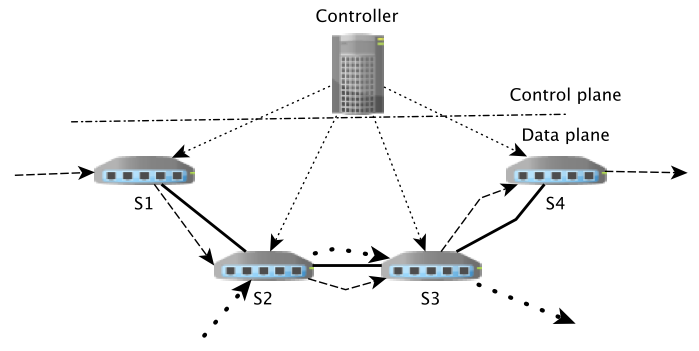
\includegraphics[width=.53\textwidth]{images/sdn.png}
	\caption{A SDN with two active flows.}
	\label{fig:sdn}
\end{figure}

Upon receiving a packet, the switch will check in its FlowTable if there is any match and perform the action associated to that match. If the receiving switch doesn't know how to forward it, it sends it to the controller that decides what to do and installs a new flow entry in the switch. Such a separation allow more flexible routing policies and ensures that adding new functions in the network is possible by simply updating the program running on the controller. The FlowTable entries can also be grouped, which will result in the switch having to chose between these entries depending on some conditions. For example, the fast reroute group will allow a switch to store alternate backup paths to provide local link protection in case of failure.

Using this approach, data plane and control plane are completely separated, as the forwarding is done by the switches, that are now simpler and cheaper, as the routing is performed by the controller. An example of such a network can be seen on the figure \ref{fig:sdn}. The straight black lines denote the physical links between the switches, thus the links inside the network. It contains two flows (the dashed and dotted lines) installed by the controller on the switches. It is worth noting that the sessions between the controller and the switches do not impose any direct connection between them and the Openflow messages could be routed across the network.

As the controller is in charge of the control plane, it is its job to deal with failures and react to their occurences. To tackle this issue, several fields must be studied. These are the detection of the failures, the protection of the links, nodes and paths, and the restoration in a stable state after a failure occured. OpenFlow does provide some protection by allowing to add in the FlowTable some fast restoration entries that can be switched to in the case of the failure of the used one. Finding efficient ways of dealing with failures remains an open problem and generates failure related papers. This survey aims at comparing several solutions in the different fields that the failure issue covers (detection, protection and restoration).

\section{Detecting failures}
There are several kind of failures that can affect a network state. Nodes can crash, links can break, resulting in flows which are no longer available. Detecting those failures plays a crucial role for the network to provide good connectivity.

This can be achieved by any agent in the network, depending on the desired performance, the available hardware and level of failures.

\subsection{Controller based detection}
A first approach is to assign the responsibility of the detection to the controller. A naive and inefficient solution would be to have it probe each switch (on each link) in the network using some kind of hello messages (LLDP\cite{5409813}, \ldots). This solution does not scale well at all\cite{6364688}, as the controller has to send a linearly increasing number of messages wrt. the link count, the node count and the flow count, this at a sufficient rate to ensure a fast enough detection.

A better approach is proposed by \cite{2013arXiv1308.4465K}. The controller computes an Eulerian cycle across all links under its responsibility, and sends a control message over that cycle using static forwarding rules pre-installed on the switches. As soon as that control message fails to come back, it can perform a binary search using another set of static rules in order to locate the link or node that has failed. A possible Eulerian cycle for the SDN in Fig.\ref{fig:sdn} can be seen on the figure \ref{fig:cycle}. As S4 and S1 are not directly connected, it is possible to create a cycle in the network without splitting the links in two (one for each direction), and then making the graph directed. This explains why S2-S3 are duplicated in the graph. In this example, we see that the controller has attached itself to the switch S2 and is sending control messages from there and waits for those to loop back in order to assess the network health.

The main limitation of this approach is that it cannot handle more than a single link or node failure, as this would break the cycle in multiple places and unlike when a single node was failing, this time the cycle would be broken at multiple places for different reasons, would render the binary search unable to detect both failures (it would only detect one).

\subsection{Switch based detection}
Another approach assigns failure detection to the switches. While these methods are usually much faster, their main drawback is that later on the controller still has to be reached in order to be notified that a failure happened, to let it respond to it, which might induce slower recovery in some cases (e.g. in small networks where LLDP could be used at a very fast rate).

Such system is presented in \cite{6364688}. This paper presents a way to monitor the health of a given tunnel at the egress side, thus in one direction. When receiving OAM messages from the switches along the tunnel, the switch is able to update its state and as soon as it has not received such message in a certain time, it can notify the controller that the path has failed.

Another solution which could be used to monitor the network health at a given time is to use BFD\cite{rfc5880} on the switches (either by piggybacking it in the data packets, or by generating new packets) and then to notify the controller in case of error.

As these methods are performed at the speed of the data plane, the detection itself is very fast, and the overhead on the network itself and on the controller is quite low. Furthermore, as Openflow is designed to be able to work on current hardware, and as current hardware usually already support BFD, performing failure detection can be performed in a SDN-agnostic way.

\begin{figure}
	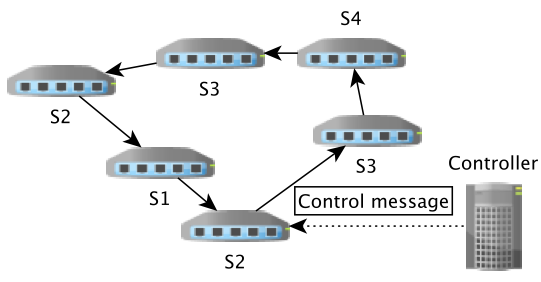
\includegraphics[width=.5\textwidth]{images/euler.png}
	\caption{An Eulerian cycle across all physical links of the network.}
	\label{fig:cycle}
\end{figure}

\section{Handling the failures}
Once a failure has been detected, the network has to react in order to be able to fulfil its role again, withstanding the failure. There are two kind of reactions which are possible, depending on the time scale at which we want the recovery to happen.

\subsection{By using path protection}
This approach consists of pre-computing backup paths for the network flows, and to install them on the switches, which can then use them as soon as a failure is detected, thus avoiding the need for any computation from the controller. Path protection in Openflow networks is achieved by using use of the fast-reroute group of flow tables. According to \cite{Sharma:2013:OMC:2445634.2445903}, using this Openflow functionality can already provide sub 50ms recovery time although this was only done in simulations.

The main issue by this techniques lies in the fact that it is not possible to install all possible backup paths for each link (or flow), as the size of the flow tables is limited.

This leads to a solution proposed in \cite{Reitblatt:2013:FDF:2491185.2491187}. It proposes a way for the network programmer to express policies on paths, which must be enforced at all time, even in case of failure (e.g. enforcing that all outgoing traffic must go through the firewall except for the DMZ). This framework then computes all possible backup paths meeting these invariants for the flows needing protection. In the end, this reduces the overall number of backup paths which have to be installed on the switches, as only the flows for which the programmer explicitly provided invariants will be protected.

A complementary approach is presented in \cite{Suchara:2011:NAJ:1993744.1993756}. This paper argues that load balancing and path protection should be treated as one problem. A management system has to compute backup paths for each flows, and those should be used all the time in order to achieve load balancing. Upon a failure, the switches will simply stop using the path that has broke and keep performing load balancing with the remaining ones. It also notifies the management system about it, which can then react to provide a more optimal routing solution in the network. This paper is independent from the routing paradigm used, but using it within SDN's is straightforward.

\subsection{By using restoration techniques}
Restoration techniques, albeit usually slower as on-the-fly computation is performed, provide the most optimal routing configuration once a failure has occurred.

There are no default restoration behaviour in Openflow: once a path has failed, the packets eventually get lost in the network until the flow gets removed from the ingress switches (which will cause a new flow computation from the controller). This is a very slow process, which will cause all the packets to be dropped until a new flow is established.

In order to achieve some form of traffic recovery, the controller has to somehow be aware of the existing flows. This is thus the network programmer task to implements error recovery mechanisms. This is precisely what \cite{Kuzniar:2013:AFR:2491185.2491218} argue against. It claims that error handling code and policies are two separate tasks, and that mixing both will increase code complexity as well as increase to risk of bugs. In order to avoid that issue, it proposes a module for the POX controller, which will perform restoration on its own, without any code from the network programmer. The principle is to record all events happening on the controller in-between failures. Once a failure occurs, it starts a new controller instance in a virtual machine, with the same topology as before minus the failed links and nodes, on top of which it replays all events it has recorded. It then finally proceeds to change the controller state to the virtual one and pushes all new flow tables. This is still an expensive process, but has the benefits of providing an optimal solution given the current network state.

Another approach which has a much lower footprint on the controller is presented in \cite{2911632}. Unlike the previous solution, this does not perform a complete recomputation of the flows. Instead it requires from the controller to remember all established paths in the network. Once a failure occurs, it then proceeds to recompute only the paths affected by the failure. It does not provide a way to perform this computation, and the obtained solution is not the optimal one as only few flows are adapted to the new network configuration. An example of this can be found from the figure \ref{fig:failures}. Supposing the network policy is optimal load balancing, if the link S1-S3 fails, \cite{2911632} will only change the flow S1-S5 and make it go through S1-S2-S5. This could result in congestion on the S1-S2 link which would violate the network policy. On the opposite, \cite{Kuzniar:2013:AFR:2491185.2491218} would have also changed the S1-S6 and make it go through S7 instead of S2.

Recently, a completely different solution was presented by \cite{Liu:2013:ECV:2482626.2482639}. It advocates for the relegation of failure recovery to the data plane. The main benefit of this lies in the fact that the data plane operates at line rate, which is much faster than the control plane. While the link connectivity itself is maintained by the data plane, the control plane is still responsible for the optimality of the paths that the data will follow across the netwok. This approach makes uses of the link reversal routing algorithm orignally presented by \cite{1094876}, adapted for the data plane (e.g. without the control messages) in order to let switches build a directed acyclic graph where the only node without outgoing link is the packet destination. It makes use of a single bit of state carried by the data packet (either piggy backed or by using two virtual links on top of a single physical interface) which is used in order to propagate whether a link has been reversed or not. The rest of the algorithm is then quite simple: upon detecting a failure preventing from forwarding the incoming packet, the switch reverses the incoming link and bounces back the packet. It is worth noting that this approach does not impose the failure detection mechanism and that there are no physical implementation of it.

\begin{figure}
	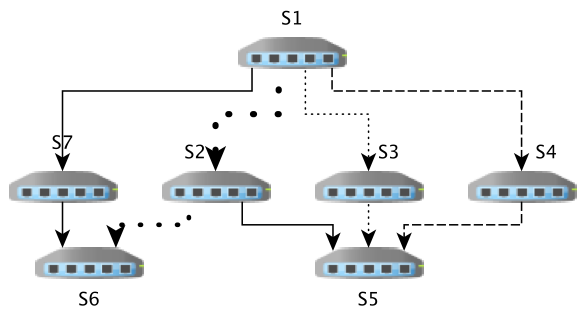
\includegraphics[width=.5\textwidth]{images/enabling_failures.png}
	\caption{An example SDN whith 3 established flows where \cite{2911632} could provide a sub-optimal recovery.}
	\label{fig:failures}
\end{figure}

\section{Conclusion}
If we were to choose a way to handle failures in the light of the approaches given in the studied papers, we would build the following aggregated solution.

For the detection step, sticking to BFD or using the solution presented in \cite{6364688} as it avoid overloading the controller with too mny control messages.

Once a failure has been detected, in order to avoid as many packet losses as possible, it would first trigger the switch to start using the flows installed in its fast-reroute FlowTable group. In order to compute those backup path the FatTire approach seems ideal \cite{Reitblatt:2013:FDF:2491185.2491187} as it proposes policies-compliant protection paths on the switches. As we are already computing additional paths for the same flows, we could also make use those in order to perform load balancing as suggested by \cite{Suchara:2011:NAJ:1993744.1993756}.

Eventually, we would use the solution presented in \cite{Kuzniar:2013:AFR:2491185.2491218} in order to perform an optimal recovery of the network.

This mixed approach allows us to detect failures quickly and to lose as few packets as possible due to the use of protection. Finally, combining the FatTire framework with the AFRO one would allow the network programmer to avoid having to deal with all the error handling code. The only part he would have to write would be to write down the network policies as well as the links requiring protection, but those are probably likely to be already defined in some other part of the network code.
\pagebreak
\bibliographystyle{IEEEtran}
\nocite{*}
\bibliography{biblio}
\end{document}